\documentclass[twoside]{book}

% Packages required by doxygen
\usepackage{fixltx2e}
\usepackage{calc}
\usepackage{doxygen}
\usepackage[export]{adjustbox} % also loads graphicx
\usepackage{graphicx}
\usepackage[utf8]{inputenc}
\usepackage{makeidx}
\usepackage{multicol}
\usepackage{multirow}
\PassOptionsToPackage{warn}{textcomp}
\usepackage{textcomp}
\usepackage[nointegrals]{wasysym}
\usepackage[table]{xcolor}

% Font selection
\usepackage[T1]{fontenc}
\usepackage[scaled=.90]{helvet}
\usepackage{courier}
\usepackage{amssymb}
\usepackage{sectsty}
\renewcommand{\familydefault}{\sfdefault}
\allsectionsfont{%
  \fontseries{bc}\selectfont%
  \color{darkgray}%
}
\renewcommand{\DoxyLabelFont}{%
  \fontseries{bc}\selectfont%
  \color{darkgray}%
}
\newcommand{\+}{\discretionary{\mbox{\scriptsize$\hookleftarrow$}}{}{}}

% Page & text layout
\usepackage{geometry}
\geometry{%
  a4paper,%
  top=2.5cm,%
  bottom=2.5cm,%
  left=2.5cm,%
  right=2.5cm%
}
\tolerance=750
\hfuzz=15pt
\hbadness=750
\setlength{\emergencystretch}{15pt}
\setlength{\parindent}{0cm}
\setlength{\parskip}{3ex plus 2ex minus 2ex}
\makeatletter
\renewcommand{\paragraph}{%
  \@startsection{paragraph}{4}{0ex}{-1.0ex}{1.0ex}{%
    \normalfont\normalsize\bfseries\SS@parafont%
  }%
}
\renewcommand{\subparagraph}{%
  \@startsection{subparagraph}{5}{0ex}{-1.0ex}{1.0ex}{%
    \normalfont\normalsize\bfseries\SS@subparafont%
  }%
}
\makeatother

% Headers & footers
\usepackage{fancyhdr}
\pagestyle{fancyplain}
\fancyhead[LE]{\fancyplain{}{\bfseries\thepage}}
\fancyhead[CE]{\fancyplain{}{}}
\fancyhead[RE]{\fancyplain{}{\bfseries\leftmark}}
\fancyhead[LO]{\fancyplain{}{\bfseries\rightmark}}
\fancyhead[CO]{\fancyplain{}{}}
\fancyhead[RO]{\fancyplain{}{\bfseries\thepage}}
\fancyfoot[LE]{\fancyplain{}{}}
\fancyfoot[CE]{\fancyplain{}{}}
\fancyfoot[RE]{\fancyplain{}{\bfseries\scriptsize Generated by Doxygen }}
\fancyfoot[LO]{\fancyplain{}{\bfseries\scriptsize Generated by Doxygen }}
\fancyfoot[CO]{\fancyplain{}{}}
\fancyfoot[RO]{\fancyplain{}{}}
\renewcommand{\footrulewidth}{0.4pt}
\renewcommand{\chaptermark}[1]{%
  \markboth{#1}{}%
}
\renewcommand{\sectionmark}[1]{%
  \markright{\thesection\ #1}%
}

% Indices & bibliography
\usepackage{natbib}
\usepackage[titles]{tocloft}
\setcounter{tocdepth}{3}
\setcounter{secnumdepth}{5}
\makeindex

% Hyperlinks (required, but should be loaded last)
\usepackage{ifpdf}
\ifpdf
  \usepackage[pdftex,pagebackref=true]{hyperref}
\else
  \usepackage[ps2pdf,pagebackref=true]{hyperref}
\fi
\hypersetup{%
  colorlinks=true,%
  linkcolor=blue,%
  citecolor=blue,%
  unicode%
}

% Custom commands
\newcommand{\clearemptydoublepage}{%
  \newpage{\pagestyle{empty}\cleardoublepage}%
}

\usepackage{caption}
\captionsetup{labelsep=space,justification=centering,font={bf},singlelinecheck=off,skip=4pt,position=top}

%===== C O N T E N T S =====

\begin{document}

% Titlepage & ToC
\hypersetup{pageanchor=false,
             bookmarksnumbered=true,
             pdfencoding=unicode
            }
\pagenumbering{alph}
\begin{titlepage}
\vspace*{7cm}
\begin{center}%
{\Large T\+E\+C\+O++ }\\
\vspace*{1cm}
{\large Generated by Doxygen 1.8.14}\\
\end{center}
\end{titlepage}
\clearemptydoublepage
\pagenumbering{roman}
\tableofcontents
\clearemptydoublepage
\pagenumbering{arabic}
\hypersetup{pageanchor=true}

%--- Begin generated contents ---
\chapter{T\+E\+C\+O++ Main page}
\label{index}\hypertarget{index}{}Main file for T\+E\+CO simulation\begin{DoxyDate}{Date}
Created on\+: 21/may/2019 
\end{DoxyDate}
\begin{DoxyAuthor}{Author}
Manfredo di Porcia \href{mailto:manfredodiporcia@gmail.com}{\tt manfredodiporcia@gmail.\+com}
\end{DoxyAuthor}
\hypertarget{index_Brief}{}\section{Brief}\label{index_Brief}
T\+E\+C\+O++ is a C++ translation of the Fortran T\+E\+CO model. ~\newline
T\+E\+CO is a Carbon transfer model introduced by Y. Luo and J. Reynolds (1999). ~\newline
Please cite original reference when using this algorithm. ~\newline
\href{https://esajournals.onlinelibrary.wiley.com/doi/10.1890/0012-9658%281999%29080%5B1568%3AVOEFCE%5D2.0.CO%3B2}{\tt https\+://esajournals.\+onlinelibrary.\+wiley.\+com/doi/10.\+1890/0012-\/9658\%281999\%29080\%5\+B1568\%3\+A\+V\+O\+E\+F\+C\+E\%5\+D2.\+0.\+C\+O\%3\+B2}

~\newline
 The equation describing the carbon transfer is the matrix representation of ~\newline
~\newline
 $ \frac{dX(t)}{dt} = BI(t) - A \xi KX(t) $

~\newline
 To compile link with Armadillo libraries (\href{http://arma.sourceforge.net/}{\tt http\+://arma.\+sourceforge.\+net/}) ~\newline
~\newline
 Test run for 10000 years with different compilers for the same code\+: ~\newline
T\+E\+C\+O++ (icpc -\/fast) -\/$>$ 9.\+112 s ~\newline
T\+E\+C\+O++ (clang++ -\/\+Ofast) -\/$>$ 8.\+689 s ~\newline
T\+E\+CO (ifort -\/fast) -\/$>$ 6.\+107 s ~\newline
~\newline
 By optimizing code (avoid repeated computation of A\+K\+\_\+inv which is constant)\+:~\newline
 T\+E\+C\+O++ (clang++ -\/\+Ofast) -\/$>$ 2.\+33873 s ~\newline

\chapter{Class Index}
\section{Class List}
Here are the classes, structs, unions and interfaces with brief descriptions\+:\begin{DoxyCompactList}
\item\contentsline{section}{\mbox{\hyperlink{class_ecosystem_carbon_state_type}{Ecosystem\+Carbon\+State\+Type}} \\*This is the main class of the T\+E\+CO model. It holds all physical variables and methods }{\pageref{class_ecosystem_carbon_state_type}}{}
\item\contentsline{section}{\mbox{\hyperlink{class_simulation_time_type}{Simulation\+Time\+Type}} \\*This class holds all the time related variables }{\pageref{class_simulation_time_type}}{}
\end{DoxyCompactList}

\chapter{File Index}
\section{File List}
Here is a list of all files with brief descriptions\+:\begin{DoxyCompactList}
\item\contentsline{section}{src/\mbox{\hyperlink{_ecosystem_carbon_state_type_8cpp}{Ecosystem\+Carbon\+State\+Type.\+cpp}} }{\pageref{_ecosystem_carbon_state_type_8cpp}}{}
\item\contentsline{section}{src/\mbox{\hyperlink{_ecosystem_carbon_state_type_8hpp}{Ecosystem\+Carbon\+State\+Type.\+hpp}} }{\pageref{_ecosystem_carbon_state_type_8hpp}}{}
\item\contentsline{section}{src/\mbox{\hyperlink{main_8cpp}{main.\+cpp}} }{\pageref{main_8cpp}}{}
\item\contentsline{section}{src/\mbox{\hyperlink{_simulation_time_type_8cpp}{Simulation\+Time\+Type.\+cpp}} }{\pageref{_simulation_time_type_8cpp}}{}
\item\contentsline{section}{src/\mbox{\hyperlink{_simulation_time_type_8hpp}{Simulation\+Time\+Type.\+hpp}} }{\pageref{_simulation_time_type_8hpp}}{}
\item\contentsline{section}{src/\mbox{\hyperlink{teco__io_8cpp}{teco\+\_\+io.\+cpp}} }{\pageref{teco__io_8cpp}}{}
\item\contentsline{section}{src/\mbox{\hyperlink{teco__io_8hpp}{teco\+\_\+io.\+hpp}} }{\pageref{teco__io_8hpp}}{}
\end{DoxyCompactList}

\chapter{Class Documentation}
\hypertarget{class_ecosystem_carbon_state_type}{}\section{Ecosystem\+Carbon\+State\+Type Class Reference}
\label{class_ecosystem_carbon_state_type}\index{Ecosystem\+Carbon\+State\+Type@{Ecosystem\+Carbon\+State\+Type}}


This is the main class of the T\+E\+CO model. It holds all physical variables and methods.  




{\ttfamily \#include $<$Ecosystem\+Carbon\+State\+Type.\+hpp$>$}

\subsection*{Public Member Functions}
\begin{DoxyCompactItemize}
\item 
\mbox{\hyperlink{class_ecosystem_carbon_state_type_a88c8eda06ce5e4bd306220280718939a}{Ecosystem\+Carbon\+State\+Type}} ()
\item 
void \mbox{\hyperlink{class_ecosystem_carbon_state_type_af8446f966b95c51b061ac5199bd8bc26}{init}} ()
\item 
void \mbox{\hyperlink{class_ecosystem_carbon_state_type_a59643b09c425cf91f8c0098d1ab491d5}{update\+\_\+\+C\+\_\+state}} ()
\item 
void \mbox{\hyperlink{class_ecosystem_carbon_state_type_af3682294ea4888ea45404b675e184bd0}{diagnostic}} ()
\item 
void \mbox{\hyperlink{class_ecosystem_carbon_state_type_a9ea22da7d71c04e00dff17a4f225855a}{matrix\+Spin\+Up}} ()
\end{DoxyCompactItemize}
\subsection*{Public Attributes}
\begin{DoxyCompactItemize}
\item 
vec \mbox{\hyperlink{class_ecosystem_carbon_state_type_a4afa44d236701692fd58577a38e5fee0}{Cpool}}
\item 
vec \mbox{\hyperlink{class_ecosystem_carbon_state_type_a1638e17e4bfc9d670ac0bd6b17296978}{Cpool\+\_\+out}}
\item 
double \mbox{\hyperlink{class_ecosystem_carbon_state_type_aa98b5ed995c5f549c37d4131487d5707}{Residence\+T\+\_\+out}} = 0.
\item 
double \mbox{\hyperlink{class_ecosystem_carbon_state_type_a83eba36ac24e57454c571f632b25c22c}{C\+Storage\+Capacity\+\_\+out}} = 0.
\item 
double \mbox{\hyperlink{class_ecosystem_carbon_state_type_a124871db6c94642d98997a081d99370b}{C\+Storage\+Potential\+\_\+out}} = 0.
\item 
double \mbox{\hyperlink{class_ecosystem_carbon_state_type_ad0ba193f2679d48489a8199c555c7598}{cinput}} = 2.\+245\+E-\/5
\end{DoxyCompactItemize}


\subsection{Detailed Description}
This is the main class of the T\+E\+CO model. It holds all physical variables and methods. 

\begin{DoxyDate}{Date}
Created on\+: 21/may/2019 
\end{DoxyDate}
\begin{DoxyAuthor}{Author}
Manfredo di Porcia 
\end{DoxyAuthor}


Definition at line 27 of file Ecosystem\+Carbon\+State\+Type.\+hpp.



\subsection{Constructor \& Destructor Documentation}
\mbox{\Hypertarget{class_ecosystem_carbon_state_type_a88c8eda06ce5e4bd306220280718939a}\label{class_ecosystem_carbon_state_type_a88c8eda06ce5e4bd306220280718939a}} 
\index{Ecosystem\+Carbon\+State\+Type@{Ecosystem\+Carbon\+State\+Type}!Ecosystem\+Carbon\+State\+Type@{Ecosystem\+Carbon\+State\+Type}}
\index{Ecosystem\+Carbon\+State\+Type@{Ecosystem\+Carbon\+State\+Type}!Ecosystem\+Carbon\+State\+Type@{Ecosystem\+Carbon\+State\+Type}}
\subsubsection{\texorpdfstring{Ecosystem\+Carbon\+State\+Type()}{EcosystemCarbonStateType()}}
{\footnotesize\ttfamily Ecosystem\+Carbon\+State\+Type\+::\+Ecosystem\+Carbon\+State\+Type (\begin{DoxyParamCaption}{ }\end{DoxyParamCaption})\hspace{0.3cm}{\ttfamily [inline]}}



Definition at line 61 of file Ecosystem\+Carbon\+State\+Type.\+hpp.



\subsection{Member Function Documentation}
\mbox{\Hypertarget{class_ecosystem_carbon_state_type_af3682294ea4888ea45404b675e184bd0}\label{class_ecosystem_carbon_state_type_af3682294ea4888ea45404b675e184bd0}} 
\index{Ecosystem\+Carbon\+State\+Type@{Ecosystem\+Carbon\+State\+Type}!diagnostic@{diagnostic}}
\index{diagnostic@{diagnostic}!Ecosystem\+Carbon\+State\+Type@{Ecosystem\+Carbon\+State\+Type}}
\subsubsection{\texorpdfstring{diagnostic()}{diagnostic()}}
{\footnotesize\ttfamily void Ecosystem\+Carbon\+State\+Type\+::diagnostic (\begin{DoxyParamCaption}{ }\end{DoxyParamCaption})}

Diagnostic 

Definition at line 45 of file Ecosystem\+Carbon\+State\+Type.\+cpp.

\mbox{\Hypertarget{class_ecosystem_carbon_state_type_af8446f966b95c51b061ac5199bd8bc26}\label{class_ecosystem_carbon_state_type_af8446f966b95c51b061ac5199bd8bc26}} 
\index{Ecosystem\+Carbon\+State\+Type@{Ecosystem\+Carbon\+State\+Type}!init@{init}}
\index{init@{init}!Ecosystem\+Carbon\+State\+Type@{Ecosystem\+Carbon\+State\+Type}}
\subsubsection{\texorpdfstring{init()}{init()}}
{\footnotesize\ttfamily void Ecosystem\+Carbon\+State\+Type\+::init (\begin{DoxyParamCaption}{ }\end{DoxyParamCaption})}

Initialize carbon state pools and matrices 

Definition at line 5 of file Ecosystem\+Carbon\+State\+Type.\+cpp.

\mbox{\Hypertarget{class_ecosystem_carbon_state_type_a9ea22da7d71c04e00dff17a4f225855a}\label{class_ecosystem_carbon_state_type_a9ea22da7d71c04e00dff17a4f225855a}} 
\index{Ecosystem\+Carbon\+State\+Type@{Ecosystem\+Carbon\+State\+Type}!matrix\+Spin\+Up@{matrix\+Spin\+Up}}
\index{matrix\+Spin\+Up@{matrix\+Spin\+Up}!Ecosystem\+Carbon\+State\+Type@{Ecosystem\+Carbon\+State\+Type}}
\subsubsection{\texorpdfstring{matrix\+Spin\+Up()}{matrixSpinUp()}}
{\footnotesize\ttfamily void Ecosystem\+Carbon\+State\+Type\+::matrix\+Spin\+Up (\begin{DoxyParamCaption}{ }\end{DoxyParamCaption})}

Semi-\/analytical spinup (?) 

Definition at line 62 of file Ecosystem\+Carbon\+State\+Type.\+cpp.

\mbox{\Hypertarget{class_ecosystem_carbon_state_type_a59643b09c425cf91f8c0098d1ab491d5}\label{class_ecosystem_carbon_state_type_a59643b09c425cf91f8c0098d1ab491d5}} 
\index{Ecosystem\+Carbon\+State\+Type@{Ecosystem\+Carbon\+State\+Type}!update\+\_\+\+C\+\_\+state@{update\+\_\+\+C\+\_\+state}}
\index{update\+\_\+\+C\+\_\+state@{update\+\_\+\+C\+\_\+state}!Ecosystem\+Carbon\+State\+Type@{Ecosystem\+Carbon\+State\+Type}}
\subsubsection{\texorpdfstring{update\+\_\+\+C\+\_\+state()}{update\_C\_state()}}
{\footnotesize\ttfamily void Ecosystem\+Carbon\+State\+Type\+::update\+\_\+\+C\+\_\+state (\begin{DoxyParamCaption}{ }\end{DoxyParamCaption})}

Main T\+E\+CO step to update carbon pools 

Definition at line 35 of file Ecosystem\+Carbon\+State\+Type.\+cpp.



\subsection{Member Data Documentation}
\mbox{\Hypertarget{class_ecosystem_carbon_state_type_ad0ba193f2679d48489a8199c555c7598}\label{class_ecosystem_carbon_state_type_ad0ba193f2679d48489a8199c555c7598}} 
\index{Ecosystem\+Carbon\+State\+Type@{Ecosystem\+Carbon\+State\+Type}!cinput@{cinput}}
\index{cinput@{cinput}!Ecosystem\+Carbon\+State\+Type@{Ecosystem\+Carbon\+State\+Type}}
\subsubsection{\texorpdfstring{cinput}{cinput}}
{\footnotesize\ttfamily double Ecosystem\+Carbon\+State\+Type\+::cinput = 2.\+245\+E-\/5}

Carbon input 

Definition at line 58 of file Ecosystem\+Carbon\+State\+Type.\+hpp.

\mbox{\Hypertarget{class_ecosystem_carbon_state_type_a4afa44d236701692fd58577a38e5fee0}\label{class_ecosystem_carbon_state_type_a4afa44d236701692fd58577a38e5fee0}} 
\index{Ecosystem\+Carbon\+State\+Type@{Ecosystem\+Carbon\+State\+Type}!Cpool@{Cpool}}
\index{Cpool@{Cpool}!Ecosystem\+Carbon\+State\+Type@{Ecosystem\+Carbon\+State\+Type}}
\subsubsection{\texorpdfstring{Cpool}{Cpool}}
{\footnotesize\ttfamily vec Ecosystem\+Carbon\+State\+Type\+::\+Cpool}

Carbon pool 

Definition at line 51 of file Ecosystem\+Carbon\+State\+Type.\+hpp.

\mbox{\Hypertarget{class_ecosystem_carbon_state_type_a1638e17e4bfc9d670ac0bd6b17296978}\label{class_ecosystem_carbon_state_type_a1638e17e4bfc9d670ac0bd6b17296978}} 
\index{Ecosystem\+Carbon\+State\+Type@{Ecosystem\+Carbon\+State\+Type}!Cpool\+\_\+out@{Cpool\+\_\+out}}
\index{Cpool\+\_\+out@{Cpool\+\_\+out}!Ecosystem\+Carbon\+State\+Type@{Ecosystem\+Carbon\+State\+Type}}
\subsubsection{\texorpdfstring{Cpool\+\_\+out}{Cpool\_out}}
{\footnotesize\ttfamily vec Ecosystem\+Carbon\+State\+Type\+::\+Cpool\+\_\+out}

Carbon pool for output 

Definition at line 52 of file Ecosystem\+Carbon\+State\+Type.\+hpp.

\mbox{\Hypertarget{class_ecosystem_carbon_state_type_a83eba36ac24e57454c571f632b25c22c}\label{class_ecosystem_carbon_state_type_a83eba36ac24e57454c571f632b25c22c}} 
\index{Ecosystem\+Carbon\+State\+Type@{Ecosystem\+Carbon\+State\+Type}!C\+Storage\+Capacity\+\_\+out@{C\+Storage\+Capacity\+\_\+out}}
\index{C\+Storage\+Capacity\+\_\+out@{C\+Storage\+Capacity\+\_\+out}!Ecosystem\+Carbon\+State\+Type@{Ecosystem\+Carbon\+State\+Type}}
\subsubsection{\texorpdfstring{C\+Storage\+Capacity\+\_\+out}{CStorageCapacity\_out}}
{\footnotesize\ttfamily double Ecosystem\+Carbon\+State\+Type\+::\+C\+Storage\+Capacity\+\_\+out = 0.}

Carbon storage capacity for output 

Definition at line 55 of file Ecosystem\+Carbon\+State\+Type.\+hpp.

\mbox{\Hypertarget{class_ecosystem_carbon_state_type_a124871db6c94642d98997a081d99370b}\label{class_ecosystem_carbon_state_type_a124871db6c94642d98997a081d99370b}} 
\index{Ecosystem\+Carbon\+State\+Type@{Ecosystem\+Carbon\+State\+Type}!C\+Storage\+Potential\+\_\+out@{C\+Storage\+Potential\+\_\+out}}
\index{C\+Storage\+Potential\+\_\+out@{C\+Storage\+Potential\+\_\+out}!Ecosystem\+Carbon\+State\+Type@{Ecosystem\+Carbon\+State\+Type}}
\subsubsection{\texorpdfstring{C\+Storage\+Potential\+\_\+out}{CStoragePotential\_out}}
{\footnotesize\ttfamily double Ecosystem\+Carbon\+State\+Type\+::\+C\+Storage\+Potential\+\_\+out = 0.}

Carbon storage potential for output 

Definition at line 56 of file Ecosystem\+Carbon\+State\+Type.\+hpp.

\mbox{\Hypertarget{class_ecosystem_carbon_state_type_aa98b5ed995c5f549c37d4131487d5707}\label{class_ecosystem_carbon_state_type_aa98b5ed995c5f549c37d4131487d5707}} 
\index{Ecosystem\+Carbon\+State\+Type@{Ecosystem\+Carbon\+State\+Type}!Residence\+T\+\_\+out@{Residence\+T\+\_\+out}}
\index{Residence\+T\+\_\+out@{Residence\+T\+\_\+out}!Ecosystem\+Carbon\+State\+Type@{Ecosystem\+Carbon\+State\+Type}}
\subsubsection{\texorpdfstring{Residence\+T\+\_\+out}{ResidenceT\_out}}
{\footnotesize\ttfamily double Ecosystem\+Carbon\+State\+Type\+::\+Residence\+T\+\_\+out = 0.}

Carbon residence time for output 

Definition at line 54 of file Ecosystem\+Carbon\+State\+Type.\+hpp.



The documentation for this class was generated from the following files\+:\begin{DoxyCompactItemize}
\item 
src/\mbox{\hyperlink{_ecosystem_carbon_state_type_8hpp}{Ecosystem\+Carbon\+State\+Type.\+hpp}}\item 
src/\mbox{\hyperlink{_ecosystem_carbon_state_type_8cpp}{Ecosystem\+Carbon\+State\+Type.\+cpp}}\end{DoxyCompactItemize}

\hypertarget{class_simulation_time_type}{}\section{Simulation\+Time\+Type Class Reference}
\label{class_simulation_time_type}\index{Simulation\+Time\+Type@{Simulation\+Time\+Type}}


This class holds all the time related variables.  




{\ttfamily \#include $<$Simulation\+Time\+Type.\+hpp$>$}

\subsection*{Public Member Functions}
\begin{DoxyCompactItemize}
\item 
void \mbox{\hyperlink{class_simulation_time_type_a271e291f8da1ae72337d456ce3899f3c}{start}} ()
\item 
bool \mbox{\hyperlink{class_simulation_time_type_a9bd3924c0990cef013132553c30eb844}{is\+\_\+end}} ()
\item 
void \mbox{\hyperlink{class_simulation_time_type_a5a0171330f407e1293c6fdf489055278}{tick\+\_\+time}} ()
\item 
void \mbox{\hyperlink{class_simulation_time_type_aa657511a4786bfd2778ce33fbaf5e3b8}{init}} (int startyr, int endyr, int nyr\+\_\+forc)
\item 
bool \mbox{\hyperlink{class_simulation_time_type_a56b971d5c4f04df090fcc7ce9764f5b9}{printC}} ()
\item 
bool \mbox{\hyperlink{class_simulation_time_type_a5ae58a97a898a812bcd24cf83ac5f6ea}{diagnostic}} ()
\item 
bool \mbox{\hyperlink{class_simulation_time_type_a3d01a0896fa801e277566bf1b2ec69d4}{is\+\_\+startof\+\_\+year}} ()
\item 
bool \mbox{\hyperlink{class_simulation_time_type_a3a35775fa077823a5849b288ae70d196}{is\+\_\+endof\+\_\+forcing}} ()
\end{DoxyCompactItemize}
\subsection*{Public Attributes}
\begin{DoxyCompactItemize}
\item 
double \mbox{\hyperlink{class_simulation_time_type_a47d3b95a336cd5be9672c48237301d4f}{dt}} = 86400.
\item 
int \mbox{\hyperlink{class_simulation_time_type_aaa632d7b7d9a2373e0e0fa8fffbbe122}{start\+Year}}
\item 
int \mbox{\hyperlink{class_simulation_time_type_af6197accafaf26492d16804698769660}{end\+Yr}}
\item 
int \mbox{\hyperlink{class_simulation_time_type_a1cd46f2a7b6924dec7aa98832a881c4e}{this\+Year}}
\item 
int \mbox{\hyperlink{class_simulation_time_type_a23da42b319f90f8ce0ea36f8c76946a5}{doy}}
\item 
chrono\+::system\+\_\+clock\+::time\+\_\+point \mbox{\hyperlink{class_simulation_time_type_a59eef0a521b5637639701bd7ad4fe73e}{sim\+\_\+time}}
\end{DoxyCompactItemize}


\subsection{Detailed Description}
This class holds all the time related variables. 

Definition at line 21 of file Simulation\+Time\+Type.\+hpp.



\subsection{Member Function Documentation}
\mbox{\Hypertarget{class_simulation_time_type_a5ae58a97a898a812bcd24cf83ac5f6ea}\label{class_simulation_time_type_a5ae58a97a898a812bcd24cf83ac5f6ea}} 
\index{Simulation\+Time\+Type@{Simulation\+Time\+Type}!diagnostic@{diagnostic}}
\index{diagnostic@{diagnostic}!Simulation\+Time\+Type@{Simulation\+Time\+Type}}
\subsubsection{\texorpdfstring{diagnostic()}{diagnostic()}}
{\footnotesize\ttfamily bool Simulation\+Time\+Type\+::diagnostic (\begin{DoxyParamCaption}{ }\end{DoxyParamCaption})\hspace{0.3cm}{\ttfamily [inline]}}

Is it time to rrun diagnostic 

Definition at line 67 of file Simulation\+Time\+Type.\+hpp.

\mbox{\Hypertarget{class_simulation_time_type_aa657511a4786bfd2778ce33fbaf5e3b8}\label{class_simulation_time_type_aa657511a4786bfd2778ce33fbaf5e3b8}} 
\index{Simulation\+Time\+Type@{Simulation\+Time\+Type}!init@{init}}
\index{init@{init}!Simulation\+Time\+Type@{Simulation\+Time\+Type}}
\subsubsection{\texorpdfstring{init()}{init()}}
{\footnotesize\ttfamily void Simulation\+Time\+Type\+::init (\begin{DoxyParamCaption}\item[{int}]{startyr,  }\item[{int}]{endyr,  }\item[{int}]{nyr\+\_\+forc }\end{DoxyParamCaption})}

init 
\begin{DoxyParams}{Parameters}
{\em startyr} & First year \\
\hline
{\em endyr} & Last year \\
\hline
{\em nyr\+\_\+forc} & Number of years of forcing \\
\hline
\end{DoxyParams}


Definition at line 3 of file Simulation\+Time\+Type.\+cpp.

\mbox{\Hypertarget{class_simulation_time_type_a9bd3924c0990cef013132553c30eb844}\label{class_simulation_time_type_a9bd3924c0990cef013132553c30eb844}} 
\index{Simulation\+Time\+Type@{Simulation\+Time\+Type}!is\+\_\+end@{is\+\_\+end}}
\index{is\+\_\+end@{is\+\_\+end}!Simulation\+Time\+Type@{Simulation\+Time\+Type}}
\subsubsection{\texorpdfstring{is\+\_\+end()}{is\_end()}}
{\footnotesize\ttfamily bool Simulation\+Time\+Type\+::is\+\_\+end (\begin{DoxyParamCaption}{ }\end{DoxyParamCaption})}

Simulation end and print execution time. \begin{DoxyReturn}{Returns}
true if simulation year is greater than last allowed year. 
\end{DoxyReturn}


Definition at line 29 of file Simulation\+Time\+Type.\+cpp.

\mbox{\Hypertarget{class_simulation_time_type_a3a35775fa077823a5849b288ae70d196}\label{class_simulation_time_type_a3a35775fa077823a5849b288ae70d196}} 
\index{Simulation\+Time\+Type@{Simulation\+Time\+Type}!is\+\_\+endof\+\_\+forcing@{is\+\_\+endof\+\_\+forcing}}
\index{is\+\_\+endof\+\_\+forcing@{is\+\_\+endof\+\_\+forcing}!Simulation\+Time\+Type@{Simulation\+Time\+Type}}
\subsubsection{\texorpdfstring{is\+\_\+endof\+\_\+forcing()}{is\_endof\_forcing()}}
{\footnotesize\ttfamily bool Simulation\+Time\+Type\+::is\+\_\+endof\+\_\+forcing (\begin{DoxyParamCaption}{ }\end{DoxyParamCaption})\hspace{0.3cm}{\ttfamily [inline]}}

Is it the end of the external forcing 

Definition at line 73 of file Simulation\+Time\+Type.\+hpp.

\mbox{\Hypertarget{class_simulation_time_type_a3d01a0896fa801e277566bf1b2ec69d4}\label{class_simulation_time_type_a3d01a0896fa801e277566bf1b2ec69d4}} 
\index{Simulation\+Time\+Type@{Simulation\+Time\+Type}!is\+\_\+startof\+\_\+year@{is\+\_\+startof\+\_\+year}}
\index{is\+\_\+startof\+\_\+year@{is\+\_\+startof\+\_\+year}!Simulation\+Time\+Type@{Simulation\+Time\+Type}}
\subsubsection{\texorpdfstring{is\+\_\+startof\+\_\+year()}{is\_startof\_year()}}
{\footnotesize\ttfamily bool Simulation\+Time\+Type\+::is\+\_\+startof\+\_\+year (\begin{DoxyParamCaption}{ }\end{DoxyParamCaption})\hspace{0.3cm}{\ttfamily [inline]}}

Is it start of the year 

Definition at line 70 of file Simulation\+Time\+Type.\+hpp.

\mbox{\Hypertarget{class_simulation_time_type_a56b971d5c4f04df090fcc7ce9764f5b9}\label{class_simulation_time_type_a56b971d5c4f04df090fcc7ce9764f5b9}} 
\index{Simulation\+Time\+Type@{Simulation\+Time\+Type}!printC@{printC}}
\index{printC@{printC}!Simulation\+Time\+Type@{Simulation\+Time\+Type}}
\subsubsection{\texorpdfstring{print\+C()}{printC()}}
{\footnotesize\ttfamily bool Simulation\+Time\+Type\+::printC (\begin{DoxyParamCaption}{ }\end{DoxyParamCaption})\hspace{0.3cm}{\ttfamily [inline]}}

Is it time to print Carbon output 

Definition at line 64 of file Simulation\+Time\+Type.\+hpp.

\mbox{\Hypertarget{class_simulation_time_type_a271e291f8da1ae72337d456ce3899f3c}\label{class_simulation_time_type_a271e291f8da1ae72337d456ce3899f3c}} 
\index{Simulation\+Time\+Type@{Simulation\+Time\+Type}!start@{start}}
\index{start@{start}!Simulation\+Time\+Type@{Simulation\+Time\+Type}}
\subsubsection{\texorpdfstring{start()}{start()}}
{\footnotesize\ttfamily void Simulation\+Time\+Type\+::start (\begin{DoxyParamCaption}{ }\end{DoxyParamCaption})}

Simulation start. 

Definition at line 23 of file Simulation\+Time\+Type.\+cpp.

\mbox{\Hypertarget{class_simulation_time_type_a5a0171330f407e1293c6fdf489055278}\label{class_simulation_time_type_a5a0171330f407e1293c6fdf489055278}} 
\index{Simulation\+Time\+Type@{Simulation\+Time\+Type}!tick\+\_\+time@{tick\+\_\+time}}
\index{tick\+\_\+time@{tick\+\_\+time}!Simulation\+Time\+Type@{Simulation\+Time\+Type}}
\subsubsection{\texorpdfstring{tick\+\_\+time()}{tick\_time()}}
{\footnotesize\ttfamily void Simulation\+Time\+Type\+::tick\+\_\+time (\begin{DoxyParamCaption}{ }\end{DoxyParamCaption})}

Advance one time step. 

Definition at line 12 of file Simulation\+Time\+Type.\+cpp.



\subsection{Member Data Documentation}
\mbox{\Hypertarget{class_simulation_time_type_a23da42b319f90f8ce0ea36f8c76946a5}\label{class_simulation_time_type_a23da42b319f90f8ce0ea36f8c76946a5}} 
\index{Simulation\+Time\+Type@{Simulation\+Time\+Type}!doy@{doy}}
\index{doy@{doy}!Simulation\+Time\+Type@{Simulation\+Time\+Type}}
\subsubsection{\texorpdfstring{doy}{doy}}
{\footnotesize\ttfamily int Simulation\+Time\+Type\+::doy}

Curent day od the year 

Definition at line 41 of file Simulation\+Time\+Type.\+hpp.

\mbox{\Hypertarget{class_simulation_time_type_a47d3b95a336cd5be9672c48237301d4f}\label{class_simulation_time_type_a47d3b95a336cd5be9672c48237301d4f}} 
\index{Simulation\+Time\+Type@{Simulation\+Time\+Type}!dt@{dt}}
\index{dt@{dt}!Simulation\+Time\+Type@{Simulation\+Time\+Type}}
\subsubsection{\texorpdfstring{dt}{dt}}
{\footnotesize\ttfamily double Simulation\+Time\+Type\+::dt = 86400.}

integration time 

Definition at line 35 of file Simulation\+Time\+Type.\+hpp.

\mbox{\Hypertarget{class_simulation_time_type_af6197accafaf26492d16804698769660}\label{class_simulation_time_type_af6197accafaf26492d16804698769660}} 
\index{Simulation\+Time\+Type@{Simulation\+Time\+Type}!end\+Yr@{end\+Yr}}
\index{end\+Yr@{end\+Yr}!Simulation\+Time\+Type@{Simulation\+Time\+Type}}
\subsubsection{\texorpdfstring{end\+Yr}{endYr}}
{\footnotesize\ttfamily int Simulation\+Time\+Type\+::end\+Yr}

Last year of simulation 

Definition at line 38 of file Simulation\+Time\+Type.\+hpp.

\mbox{\Hypertarget{class_simulation_time_type_a59eef0a521b5637639701bd7ad4fe73e}\label{class_simulation_time_type_a59eef0a521b5637639701bd7ad4fe73e}} 
\index{Simulation\+Time\+Type@{Simulation\+Time\+Type}!sim\+\_\+time@{sim\+\_\+time}}
\index{sim\+\_\+time@{sim\+\_\+time}!Simulation\+Time\+Type@{Simulation\+Time\+Type}}
\subsubsection{\texorpdfstring{sim\+\_\+time}{sim\_time}}
{\footnotesize\ttfamily chrono\+::system\+\_\+clock\+::time\+\_\+point Simulation\+Time\+Type\+::sim\+\_\+time}

Main loop duration 

Definition at line 43 of file Simulation\+Time\+Type.\+hpp.

\mbox{\Hypertarget{class_simulation_time_type_aaa632d7b7d9a2373e0e0fa8fffbbe122}\label{class_simulation_time_type_aaa632d7b7d9a2373e0e0fa8fffbbe122}} 
\index{Simulation\+Time\+Type@{Simulation\+Time\+Type}!start\+Year@{start\+Year}}
\index{start\+Year@{start\+Year}!Simulation\+Time\+Type@{Simulation\+Time\+Type}}
\subsubsection{\texorpdfstring{start\+Year}{startYear}}
{\footnotesize\ttfamily int Simulation\+Time\+Type\+::start\+Year}

First year of simulation 

Definition at line 37 of file Simulation\+Time\+Type.\+hpp.

\mbox{\Hypertarget{class_simulation_time_type_a1cd46f2a7b6924dec7aa98832a881c4e}\label{class_simulation_time_type_a1cd46f2a7b6924dec7aa98832a881c4e}} 
\index{Simulation\+Time\+Type@{Simulation\+Time\+Type}!this\+Year@{this\+Year}}
\index{this\+Year@{this\+Year}!Simulation\+Time\+Type@{Simulation\+Time\+Type}}
\subsubsection{\texorpdfstring{this\+Year}{thisYear}}
{\footnotesize\ttfamily int Simulation\+Time\+Type\+::this\+Year}

Current year 

Definition at line 40 of file Simulation\+Time\+Type.\+hpp.



The documentation for this class was generated from the following files\+:\begin{DoxyCompactItemize}
\item 
src/\mbox{\hyperlink{_simulation_time_type_8hpp}{Simulation\+Time\+Type.\+hpp}}\item 
src/\mbox{\hyperlink{_simulation_time_type_8cpp}{Simulation\+Time\+Type.\+cpp}}\end{DoxyCompactItemize}

\chapter{File Documentation}
\hypertarget{_ecosystem_carbon_state_type_8cpp}{}\section{src/\+Ecosystem\+Carbon\+State\+Type.cpp File Reference}
\label{_ecosystem_carbon_state_type_8cpp}\index{src/\+Ecosystem\+Carbon\+State\+Type.\+cpp@{src/\+Ecosystem\+Carbon\+State\+Type.\+cpp}}
{\ttfamily \#include \char`\"{}Ecosystem\+Carbon\+State\+Type.\+hpp\char`\"{}}\newline
{\ttfamily \#include \char`\"{}Simulation\+Time\+Type.\+hpp\char`\"{}}\newline
Include dependency graph for Ecosystem\+Carbon\+State\+Type.\+cpp\+:\nopagebreak
\begin{figure}[H]
\begin{center}
\leavevmode
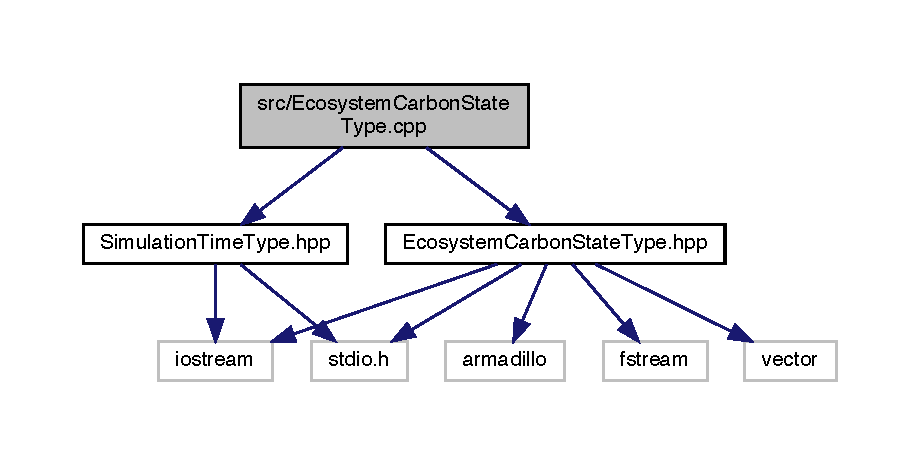
\includegraphics[width=350pt]{_ecosystem_carbon_state_type_8cpp__incl}
\end{center}
\end{figure}
\subsection*{Variables}
\begin{DoxyCompactItemize}
\item 
\mbox{\hyperlink{class_simulation_time_type}{Simulation\+Time\+Type}} \mbox{\hyperlink{_ecosystem_carbon_state_type_8cpp_a29061a5b4013676328dd5f8f67795934}{Time}}
\end{DoxyCompactItemize}


\subsection{Variable Documentation}
\mbox{\Hypertarget{_ecosystem_carbon_state_type_8cpp_a29061a5b4013676328dd5f8f67795934}\label{_ecosystem_carbon_state_type_8cpp_a29061a5b4013676328dd5f8f67795934}} 
\index{Ecosystem\+Carbon\+State\+Type.\+cpp@{Ecosystem\+Carbon\+State\+Type.\+cpp}!Time@{Time}}
\index{Time@{Time}!Ecosystem\+Carbon\+State\+Type.\+cpp@{Ecosystem\+Carbon\+State\+Type.\+cpp}}
\subsubsection{\texorpdfstring{Time}{Time}}
{\footnotesize\ttfamily \mbox{\hyperlink{class_simulation_time_type}{Simulation\+Time\+Type}} Time}


\hypertarget{_ecosystem_carbon_state_type_8hpp}{}\section{src/\+Ecosystem\+Carbon\+State\+Type.hpp File Reference}
\label{_ecosystem_carbon_state_type_8hpp}\index{src/\+Ecosystem\+Carbon\+State\+Type.\+hpp@{src/\+Ecosystem\+Carbon\+State\+Type.\+hpp}}
{\ttfamily \#include \char`\"{}armadillo\char`\"{}}\newline
{\ttfamily \#include $<$stdio.\+h$>$}\newline
{\ttfamily \#include $<$fstream$>$}\newline
{\ttfamily \#include $<$iostream$>$}\newline
{\ttfamily \#include $<$vector$>$}\newline
Include dependency graph for Ecosystem\+Carbon\+State\+Type.\+hpp\+:\nopagebreak
\begin{figure}[H]
\begin{center}
\leavevmode
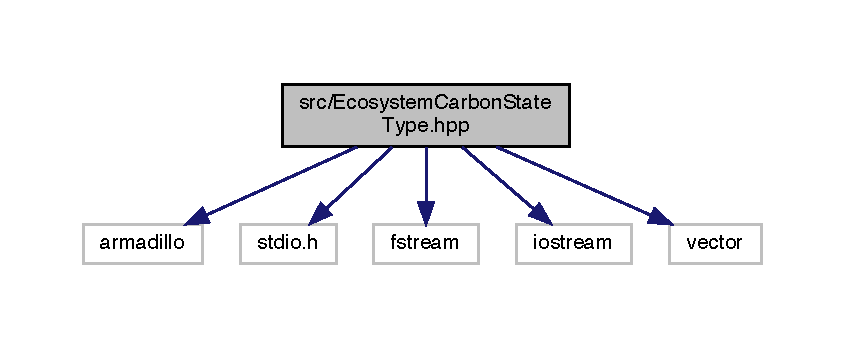
\includegraphics[width=350pt]{_ecosystem_carbon_state_type_8hpp__incl}
\end{center}
\end{figure}
This graph shows which files directly or indirectly include this file\+:\nopagebreak
\begin{figure}[H]
\begin{center}
\leavevmode
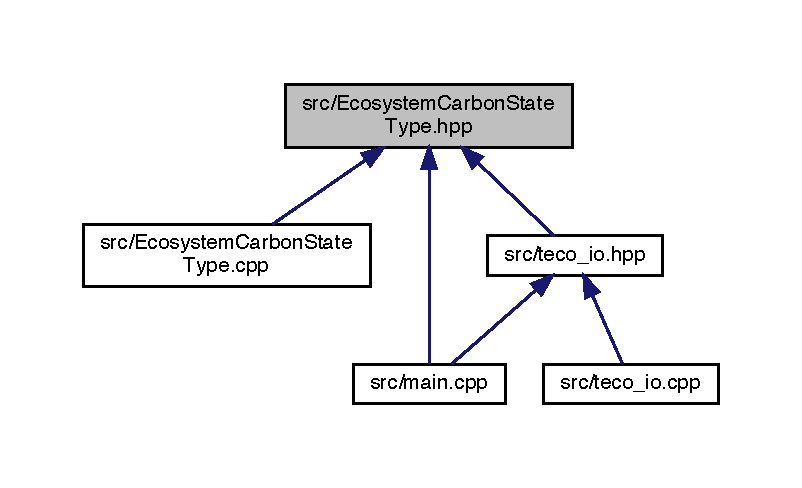
\includegraphics[width=350pt]{_ecosystem_carbon_state_type_8hpp__dep__incl}
\end{center}
\end{figure}
\subsection*{Classes}
\begin{DoxyCompactItemize}
\item 
class \mbox{\hyperlink{class_ecosystem_carbon_state_type}{Ecosystem\+Carbon\+State\+Type}}
\begin{DoxyCompactList}\small\item\em This is the main class of the T\+E\+CO model. It holds all physical variables and methods. \end{DoxyCompactList}\end{DoxyCompactItemize}
\subsection*{Macros}
\begin{DoxyCompactItemize}
\item 
\#define \mbox{\hyperlink{_ecosystem_carbon_state_type_8hpp_abadef0895f9337ae87c1ec5a4f4fc937}{npools}}~7
\item 
\#define \mbox{\hyperlink{_ecosystem_carbon_state_type_8hpp_a719a66772595ff7009bcdbf069a64334}{sec\+\_\+in\+\_\+y}}~(365 $\ast$ 24 $\ast$ 3600.)
\end{DoxyCompactItemize}


\subsection{Macro Definition Documentation}
\mbox{\Hypertarget{_ecosystem_carbon_state_type_8hpp_abadef0895f9337ae87c1ec5a4f4fc937}\label{_ecosystem_carbon_state_type_8hpp_abadef0895f9337ae87c1ec5a4f4fc937}} 
\index{Ecosystem\+Carbon\+State\+Type.\+hpp@{Ecosystem\+Carbon\+State\+Type.\+hpp}!npools@{npools}}
\index{npools@{npools}!Ecosystem\+Carbon\+State\+Type.\+hpp@{Ecosystem\+Carbon\+State\+Type.\+hpp}}
\subsubsection{\texorpdfstring{npools}{npools}}
{\footnotesize\ttfamily \#define npools~7}

Total number of carbon pools 

Definition at line 15 of file Ecosystem\+Carbon\+State\+Type.\+hpp.

\mbox{\Hypertarget{_ecosystem_carbon_state_type_8hpp_a719a66772595ff7009bcdbf069a64334}\label{_ecosystem_carbon_state_type_8hpp_a719a66772595ff7009bcdbf069a64334}} 
\index{Ecosystem\+Carbon\+State\+Type.\+hpp@{Ecosystem\+Carbon\+State\+Type.\+hpp}!sec\+\_\+in\+\_\+y@{sec\+\_\+in\+\_\+y}}
\index{sec\+\_\+in\+\_\+y@{sec\+\_\+in\+\_\+y}!Ecosystem\+Carbon\+State\+Type.\+hpp@{Ecosystem\+Carbon\+State\+Type.\+hpp}}
\subsubsection{\texorpdfstring{sec\+\_\+in\+\_\+y}{sec\_in\_y}}
{\footnotesize\ttfamily \#define sec\+\_\+in\+\_\+y~(365 $\ast$ 24 $\ast$ 3600.)}

Number of second in one year 

Definition at line 16 of file Ecosystem\+Carbon\+State\+Type.\+hpp.


\hypertarget{main_8cpp}{}\section{src/main.cpp File Reference}
\label{main_8cpp}\index{src/main.\+cpp@{src/main.\+cpp}}
{\ttfamily \#include $<$iostream$>$}\newline
{\ttfamily \#include \char`\"{}Ecosystem\+Carbon\+State\+Type.\+hpp\char`\"{}}\newline
{\ttfamily \#include \char`\"{}teco\+\_\+io.\+hpp\char`\"{}}\newline
{\ttfamily \#include \char`\"{}Simulation\+Time\+Type.\+hpp\char`\"{}}\newline
Include dependency graph for main.\+cpp\+:\nopagebreak
\begin{figure}[H]
\begin{center}
\leavevmode
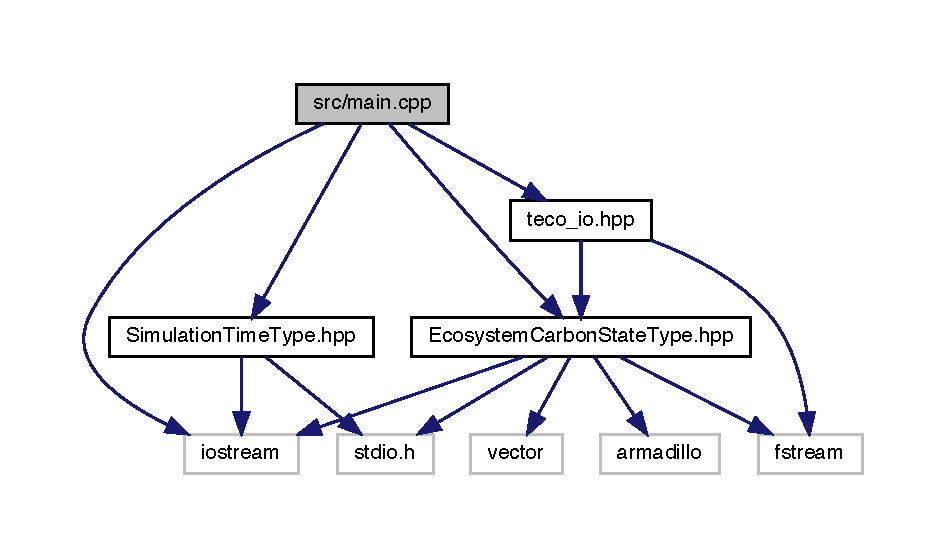
\includegraphics[width=350pt]{main_8cpp__incl}
\end{center}
\end{figure}
\subsection*{Functions}
\begin{DoxyCompactItemize}
\item 
int \mbox{\hyperlink{main_8cpp_ac0f2228420376f4db7e1274f2b41667c}{main}} (int argc, const char $\ast$argv\mbox{[}$\,$\mbox{]})
\end{DoxyCompactItemize}


\subsection{Function Documentation}
\mbox{\Hypertarget{main_8cpp_ac0f2228420376f4db7e1274f2b41667c}\label{main_8cpp_ac0f2228420376f4db7e1274f2b41667c}} 
\index{main.\+cpp@{main.\+cpp}!main@{main}}
\index{main@{main}!main.\+cpp@{main.\+cpp}}
\subsubsection{\texorpdfstring{main()}{main()}}
{\footnotesize\ttfamily int main (\begin{DoxyParamCaption}\item[{int}]{argc,  }\item[{const char $\ast$}]{argv\mbox{[}$\,$\mbox{]} }\end{DoxyParamCaption})}


\hypertarget{_simulation_time_type_8cpp}{}\section{src/\+Simulation\+Time\+Type.cpp File Reference}
\label{_simulation_time_type_8cpp}\index{src/\+Simulation\+Time\+Type.\+cpp@{src/\+Simulation\+Time\+Type.\+cpp}}
{\ttfamily \#include \char`\"{}Simulation\+Time\+Type.\+hpp\char`\"{}}\newline
Include dependency graph for Simulation\+Time\+Type.\+cpp\+:\nopagebreak
\begin{figure}[H]
\begin{center}
\leavevmode
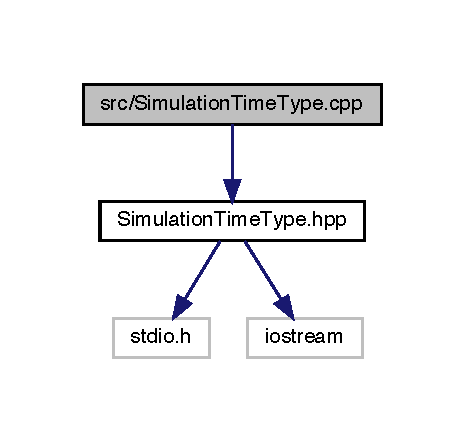
\includegraphics[width=223pt]{_simulation_time_type_8cpp__incl}
\end{center}
\end{figure}

\hypertarget{_simulation_time_type_8hpp}{}\section{src/\+Simulation\+Time\+Type.hpp File Reference}
\label{_simulation_time_type_8hpp}\index{src/\+Simulation\+Time\+Type.\+hpp@{src/\+Simulation\+Time\+Type.\+hpp}}
{\ttfamily \#include $<$stdio.\+h$>$}\newline
{\ttfamily \#include $<$iostream$>$}\newline
Include dependency graph for Simulation\+Time\+Type.\+hpp\+:\nopagebreak
\begin{figure}[H]
\begin{center}
\leavevmode
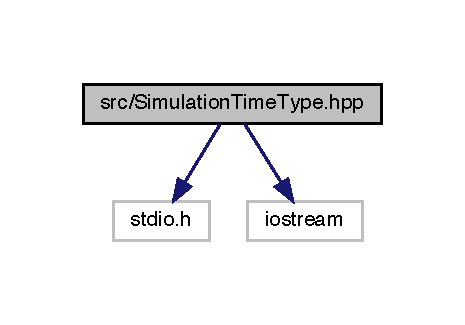
\includegraphics[width=223pt]{_simulation_time_type_8hpp__incl}
\end{center}
\end{figure}
This graph shows which files directly or indirectly include this file\+:\nopagebreak
\begin{figure}[H]
\begin{center}
\leavevmode
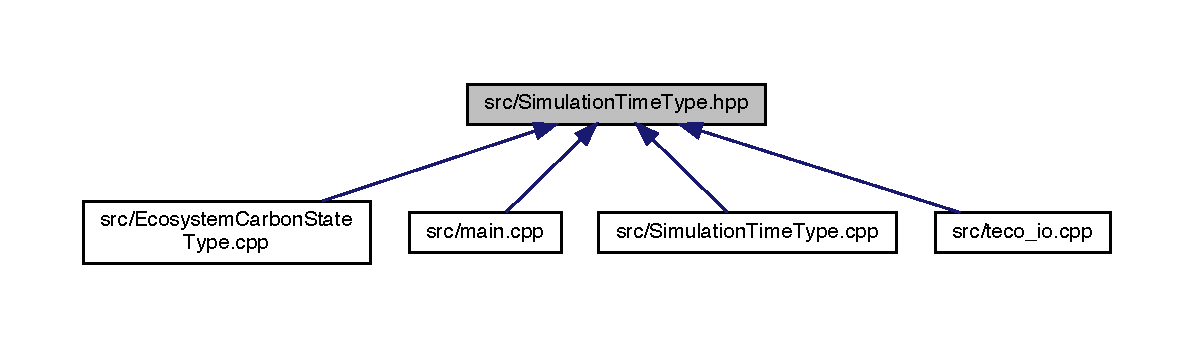
\includegraphics[width=350pt]{_simulation_time_type_8hpp__dep__incl}
\end{center}
\end{figure}
\subsection*{Classes}
\begin{DoxyCompactItemize}
\item 
class \mbox{\hyperlink{class_simulation_time_type}{Simulation\+Time\+Type}}
\begin{DoxyCompactList}\small\item\em This class holds all the time related variables. \end{DoxyCompactList}\end{DoxyCompactItemize}
\subsection*{Variables}
\begin{DoxyCompactItemize}
\item 
\mbox{\hyperlink{class_simulation_time_type}{Simulation\+Time\+Type}} \mbox{\hyperlink{_simulation_time_type_8hpp_a29061a5b4013676328dd5f8f67795934}{Time}}
\end{DoxyCompactItemize}


\subsection{Detailed Description}
\begin{DoxyDate}{Date}
Created on\+: 21/may/2019 
\end{DoxyDate}
\begin{DoxyAuthor}{Author}
Manfredo di Porcia 
\end{DoxyAuthor}


\subsection{Variable Documentation}
\mbox{\Hypertarget{_simulation_time_type_8hpp_a29061a5b4013676328dd5f8f67795934}\label{_simulation_time_type_8hpp_a29061a5b4013676328dd5f8f67795934}} 
\index{Simulation\+Time\+Type.\+hpp@{Simulation\+Time\+Type.\+hpp}!Time@{Time}}
\index{Time@{Time}!Simulation\+Time\+Type.\+hpp@{Simulation\+Time\+Type.\+hpp}}
\subsubsection{\texorpdfstring{Time}{Time}}
{\footnotesize\ttfamily \mbox{\hyperlink{class_simulation_time_type}{Simulation\+Time\+Type}} Time}



Definition at line 3 of file Ecosystem\+Carbon\+State\+Type.\+cpp.


\hypertarget{teco__io_8cpp}{}\section{src/teco\+\_\+io.cpp File Reference}
\label{teco__io_8cpp}\index{src/teco\+\_\+io.\+cpp@{src/teco\+\_\+io.\+cpp}}
{\ttfamily \#include \char`\"{}teco\+\_\+io.\+hpp\char`\"{}}\newline
{\ttfamily \#include \char`\"{}Simulation\+Time\+Type.\+hpp\char`\"{}}\newline
Include dependency graph for teco\+\_\+io.\+cpp\+:\nopagebreak
\begin{figure}[H]
\begin{center}
\leavevmode
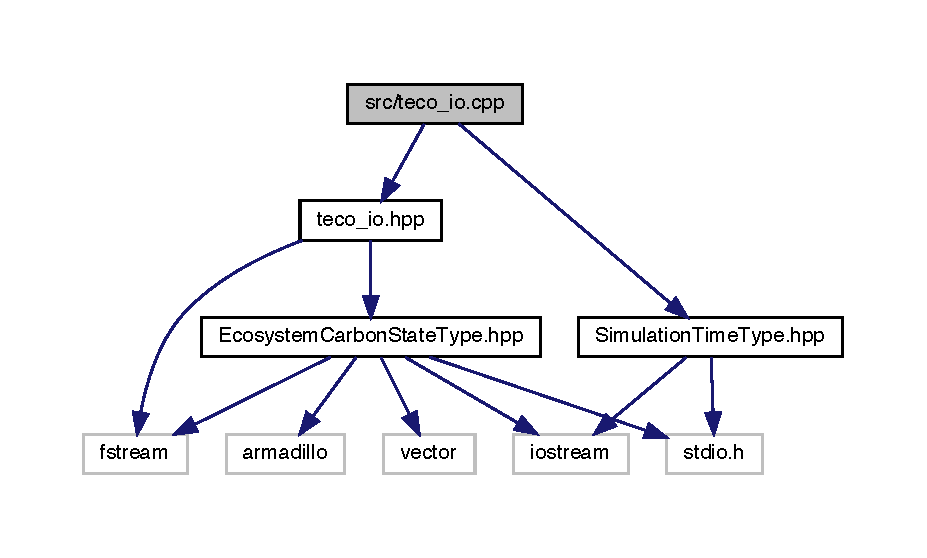
\includegraphics[width=350pt]{teco__io_8cpp__incl}
\end{center}
\end{figure}
\subsection*{Functions}
\begin{DoxyCompactItemize}
\item 
void \mbox{\hyperlink{teco__io_8cpp_a2a23e02bb3674581328d65788c1d1c24}{write\+\_\+header}} (ofstream \&myfile)
\item 
void \mbox{\hyperlink{teco__io_8cpp_a896db640499427e8794814e3c68c8b8d}{write\+\_\+c\+\_\+state}} (ofstream \&outfile, \mbox{\hyperlink{class_ecosystem_carbon_state_type}{Ecosystem\+Carbon\+State\+Type}} \&my\+\_\+state)
\item 
void \mbox{\hyperlink{teco__io_8cpp_aee5474a798255fc8604ad3ae50117cc4}{read\+\_\+inputF}} (ifstream \&infile)
\end{DoxyCompactItemize}


\subsection{Function Documentation}
\mbox{\Hypertarget{teco__io_8cpp_aee5474a798255fc8604ad3ae50117cc4}\label{teco__io_8cpp_aee5474a798255fc8604ad3ae50117cc4}} 
\index{teco\+\_\+io.\+cpp@{teco\+\_\+io.\+cpp}!read\+\_\+inputF@{read\+\_\+inputF}}
\index{read\+\_\+inputF@{read\+\_\+inputF}!teco\+\_\+io.\+cpp@{teco\+\_\+io.\+cpp}}
\subsubsection{\texorpdfstring{read\+\_\+input\+F()}{read\_inputF()}}
{\footnotesize\ttfamily void read\+\_\+inputF (\begin{DoxyParamCaption}\item[{ifstream \&}]{infile }\end{DoxyParamCaption})}

\mbox{\Hypertarget{teco__io_8cpp_a896db640499427e8794814e3c68c8b8d}\label{teco__io_8cpp_a896db640499427e8794814e3c68c8b8d}} 
\index{teco\+\_\+io.\+cpp@{teco\+\_\+io.\+cpp}!write\+\_\+c\+\_\+state@{write\+\_\+c\+\_\+state}}
\index{write\+\_\+c\+\_\+state@{write\+\_\+c\+\_\+state}!teco\+\_\+io.\+cpp@{teco\+\_\+io.\+cpp}}
\subsubsection{\texorpdfstring{write\+\_\+c\+\_\+state()}{write\_c\_state()}}
{\footnotesize\ttfamily void write\+\_\+c\+\_\+state (\begin{DoxyParamCaption}\item[{ofstream \&}]{outfile,  }\item[{\mbox{\hyperlink{class_ecosystem_carbon_state_type}{Ecosystem\+Carbon\+State\+Type}} \&}]{my\+\_\+state }\end{DoxyParamCaption})}

\mbox{\Hypertarget{teco__io_8cpp_a2a23e02bb3674581328d65788c1d1c24}\label{teco__io_8cpp_a2a23e02bb3674581328d65788c1d1c24}} 
\index{teco\+\_\+io.\+cpp@{teco\+\_\+io.\+cpp}!write\+\_\+header@{write\+\_\+header}}
\index{write\+\_\+header@{write\+\_\+header}!teco\+\_\+io.\+cpp@{teco\+\_\+io.\+cpp}}
\subsubsection{\texorpdfstring{write\+\_\+header()}{write\_header()}}
{\footnotesize\ttfamily void write\+\_\+header (\begin{DoxyParamCaption}\item[{ofstream \&}]{myfile }\end{DoxyParamCaption})}


\hypertarget{teco__io_8hpp}{}\section{src/teco\+\_\+io.hpp File Reference}
\label{teco__io_8hpp}\index{src/teco\+\_\+io.\+hpp@{src/teco\+\_\+io.\+hpp}}
{\ttfamily \#include $<$fstream$>$}\newline
{\ttfamily \#include \char`\"{}Ecosystem\+Carbon\+State\+Type.\+hpp\char`\"{}}\newline
Include dependency graph for teco\+\_\+io.\+hpp\+:\nopagebreak
\begin{figure}[H]
\begin{center}
\leavevmode
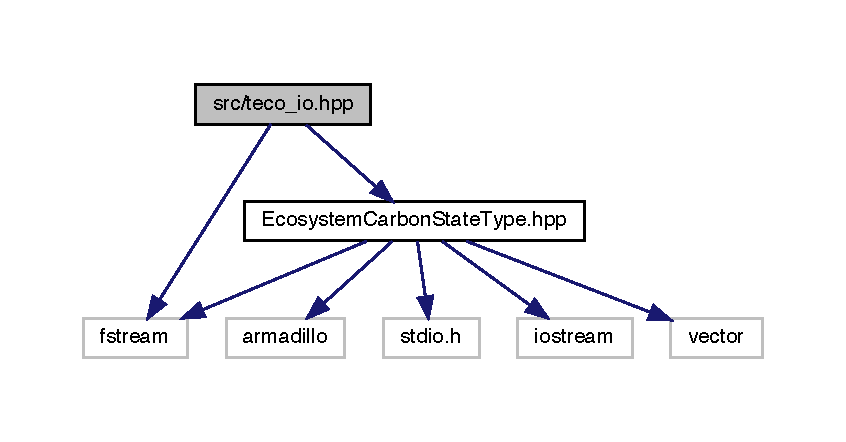
\includegraphics[width=350pt]{teco__io_8hpp__incl}
\end{center}
\end{figure}
This graph shows which files directly or indirectly include this file\+:\nopagebreak
\begin{figure}[H]
\begin{center}
\leavevmode
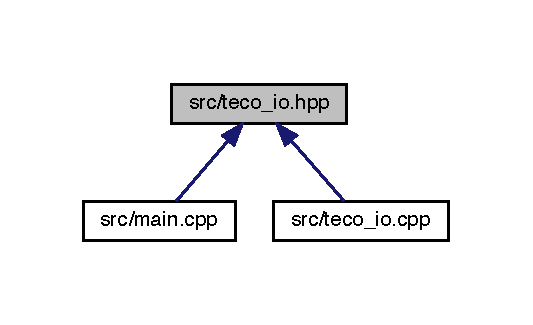
\includegraphics[width=256pt]{teco__io_8hpp__dep__incl}
\end{center}
\end{figure}
\subsection*{Functions}
\begin{DoxyCompactItemize}
\item 
void \mbox{\hyperlink{teco__io_8hpp_a3653400fa821dcfaa304a6b1dc8eba33}{read\+\_\+inputF}} (ifstream \&)
\item 
void \mbox{\hyperlink{teco__io_8hpp_a840a9d4e8a7c5afa631c74e612dc51e9}{write\+\_\+header}} (ofstream \&)
\item 
void \mbox{\hyperlink{teco__io_8hpp_a417465eff4ddf375a4ceecfe2a3af9e1}{write\+\_\+c\+\_\+state}} (ofstream \&, \mbox{\hyperlink{class_ecosystem_carbon_state_type}{Ecosystem\+Carbon\+State\+Type}} \&)
\end{DoxyCompactItemize}


\subsection{Function Documentation}
\mbox{\Hypertarget{teco__io_8hpp_a3653400fa821dcfaa304a6b1dc8eba33}\label{teco__io_8hpp_a3653400fa821dcfaa304a6b1dc8eba33}} 
\index{teco\+\_\+io.\+hpp@{teco\+\_\+io.\+hpp}!read\+\_\+inputF@{read\+\_\+inputF}}
\index{read\+\_\+inputF@{read\+\_\+inputF}!teco\+\_\+io.\+hpp@{teco\+\_\+io.\+hpp}}
\subsubsection{\texorpdfstring{read\+\_\+input\+F()}{read\_inputF()}}
{\footnotesize\ttfamily void read\+\_\+inputF (\begin{DoxyParamCaption}\item[{ifstream \&}]{ }\end{DoxyParamCaption})}



Definition at line 17 of file teco\+\_\+io.\+cpp.

\mbox{\Hypertarget{teco__io_8hpp_a417465eff4ddf375a4ceecfe2a3af9e1}\label{teco__io_8hpp_a417465eff4ddf375a4ceecfe2a3af9e1}} 
\index{teco\+\_\+io.\+hpp@{teco\+\_\+io.\+hpp}!write\+\_\+c\+\_\+state@{write\+\_\+c\+\_\+state}}
\index{write\+\_\+c\+\_\+state@{write\+\_\+c\+\_\+state}!teco\+\_\+io.\+hpp@{teco\+\_\+io.\+hpp}}
\subsubsection{\texorpdfstring{write\+\_\+c\+\_\+state()}{write\_c\_state()}}
{\footnotesize\ttfamily void write\+\_\+c\+\_\+state (\begin{DoxyParamCaption}\item[{ofstream \&}]{,  }\item[{\mbox{\hyperlink{class_ecosystem_carbon_state_type}{Ecosystem\+Carbon\+State\+Type}} \&}]{ }\end{DoxyParamCaption})}



Definition at line 10 of file teco\+\_\+io.\+cpp.

\mbox{\Hypertarget{teco__io_8hpp_a840a9d4e8a7c5afa631c74e612dc51e9}\label{teco__io_8hpp_a840a9d4e8a7c5afa631c74e612dc51e9}} 
\index{teco\+\_\+io.\+hpp@{teco\+\_\+io.\+hpp}!write\+\_\+header@{write\+\_\+header}}
\index{write\+\_\+header@{write\+\_\+header}!teco\+\_\+io.\+hpp@{teco\+\_\+io.\+hpp}}
\subsubsection{\texorpdfstring{write\+\_\+header()}{write\_header()}}
{\footnotesize\ttfamily void write\+\_\+header (\begin{DoxyParamCaption}\item[{ofstream \&}]{ }\end{DoxyParamCaption})}



Definition at line 4 of file teco\+\_\+io.\+cpp.


%--- End generated contents ---

% Index
\backmatter
\newpage
\phantomsection
\clearemptydoublepage
\addcontentsline{toc}{chapter}{Index}
\printindex

\end{document}
